\subsection{Protein expression}
Protein expression is the process by which protein is synthesised using the information in the messenger RNA (mRNA) (Figure \ref{fig:tranc_transl}). 


\begin{figure}[htbp!]
\center
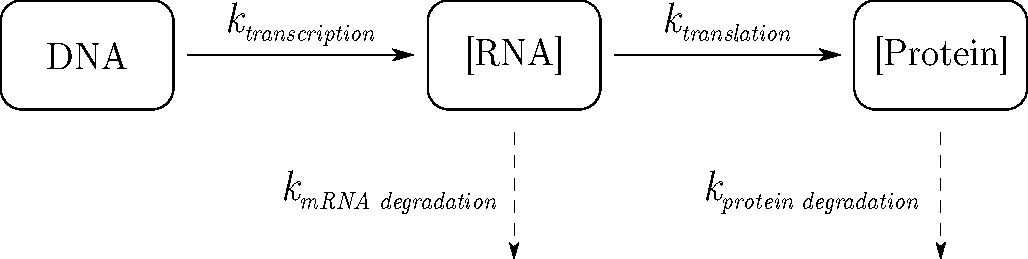
\includegraphics[width=0.7\textwidth]{chapters/Introduction/Figures/transc_transl.pdf}
\caption[Protein expression depends on the rates of RNA and protein synthesis and their degradation.]{\textbf{Protein expression depends on the rates of RNA and protein synthesis and their degradation.} Solid arrow represents synthesis whereas dashed arrow represents degradation. [RNA], concentration of mRNA; [Protein], concentration of protein; $k_{transcription}$, rate of transcription; $k_{translation}$, rate of translation; $k_{mRNA\ degradation}$, rate of mRNA degradation; $k_{protein\ degradation}$, rate of protein degradation. Figure redrawn from Abreu \textit{et al.} (2009).}%the List of Figures because of the *}
\label{fig:tranc_transl}
\end{figure}

Intuitively, we expect the protein yield to be predictable using mRNA levels, the correlation is lower than expected \cite{Abreu2009-zf, Taniguchi2010-uq, Bernstein2002-gg}. This reflects the complexities of the underlying process. The amount of protein produced is determined by translation rate and protein degradation (Figure \ref{fig:tranc_transl}).  This dynamic system can be mathematically described by a first order differential equation \cite{Abreu2009-zf} whose solution at equilibrium gives the following relationship relationship between protein concentration $(P_{\infty})$, mRNA concentration $(R_{\infty})$, translation rate $(k_{translation})$ and protein degradation rate $(k_{protein\ degradation})$ :

\begin{equation}
    \frac{P_{\infty}}{R_\infty} = \frac{k_{translation}}{k_{protein\ degradation}}
\end{equation}

There are various mechanisms regulating translation and protein degradation, so the correlation between $(P_{\infty})$ and $(R_{\infty})$ is not perfect. Squared Pearson's correlation is around $0.4$ for many organisms \cite{Abreu2009-zf}. Assuming the protein degradation rate $(k_{protein\ degradation})$ to be a constant, the ratio of $P/R$ depends upon the translation rate $(k_{translation})$ only. Hence, the amount of protein can be modulated by tuning  $k_{translation}$.

\subsection{Translation}

Translation in prokaryotes is \textit{initiated} when the small ribosome subunit $30S$ binds to the Shine-Dalgarno sequence and moves upto the start codon. The currently accepted model is that the initiator tRNA charged with N-formylmethionine, initiation factor (IF-2) and guanosine triphosphate (GTP) binds with this subunit followed by the release of IF-3 \cite{hames2005biochemistry}. This complex is called the 30S initiation complex. IF-1 and IF-2 are released and the large ribosomal subunit $50S$ now binds followed by the hydrolysis of GTP, to form a $70S$ initiation complex. 

After the formation of initiation complex, the decoding of information in the mRNA begins. This is called \textit{translation elongation}. The $70S$ complex consists of three active sites: peptidyl-tRNA site (P site), aminoacyl-tRNA site (A site) and exit site (E site). Initially, the start codon and the successive codon of mRNA is positioned at P site and A site respectively. The initiator tRNA charged with N-formylmethionine is coupled with start codon at the P site and the corresponding aminoacyl-tRNA is coupled to the next codon at the A site through codon-anticodon pairing (Figure \ref{fig:prokaryotic_translation}). Peptide bond is formed between the amino acid carried by tRNA at P and A site to give a dipeptide. tRNA at P site is translocated to E site, tRNA at A site to P site and the ribosome moves along the mRNA. The deactylated tRNA at E site is released. Since the A site is now empty, it receives the next aminoacyl-tRNA and the process continues adding an amino acid to C terminal of the dipeptide. 


Once the ribosome encounters a stop codon, release factor (RF1 or RF2 and RF3) bind to the ribosome resulting in a tranfer of polypeptide to a water molecule rather than aminoacyl-tRNA. The free polypeptide is released from the ribosome and $70S$ ribosome disassociates into $30S$ and $50S$ subunits. This step is called \textit{translation termination}. 

%%TODO - FIGURE FOR TRANSLATION


\begin{figure}[!hbtp]
    \centering
    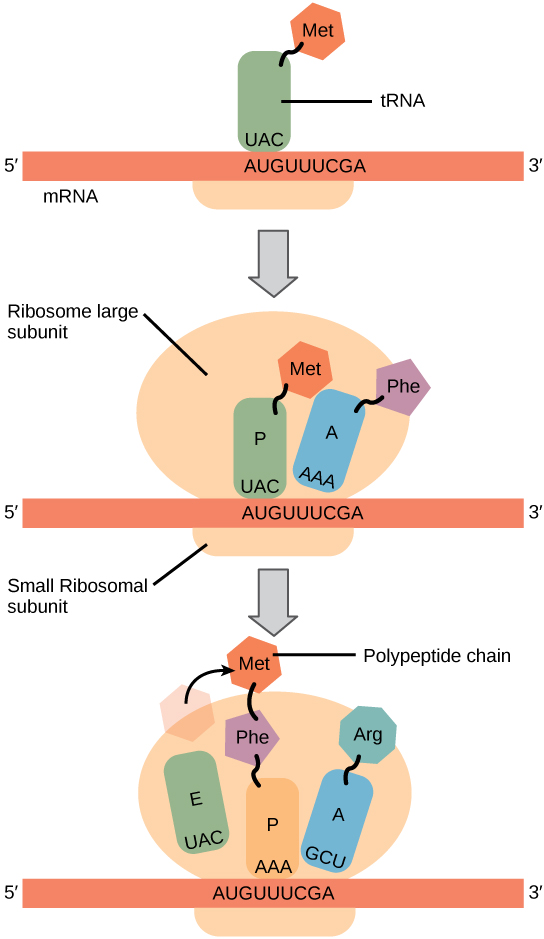
\includegraphics{chapters/Introduction/Figures/translation.jpg}
    \caption[Prokaryotic translation.]{\textbf{Prokaryotic translation.} Initiator tRNA binds to the smaller subunit at the start codon. Larger subunit joins to form a translation initiation complex such that initiator tRNA is at P site and the next aminoacyl-tRNA is at A site. Initiator tRNA moves to the E site, dipeptide is formed at the P site and new aminoacyl-tRNA is received at the A site. Figure from OpenStax College, Concepts of Biology. OpenStax CNX (Creative Commons license: CC BY 4.0) }%the List of Figures because of the *}
    \label{fig:prokaryotic_translation}
\end{figure}


\subsection{mRNA features and their roles in translation}
Translation rate may depend on the rate formation of translation initiation complex and utilisation of available tRNA pool. Several features of a mRNA sequence are suggested to explain these two major dependencies of translation rate. However, many mRNA features are not independent, making it hard to distinguish the impacts of individual features \cite{mauger2019mrna}. The main features that have been considered to date, can be classified into three categories: codon preferences, mRNA folding (secondary structure) and mRNA:ncRNA avoidance. These three categories of features is the basis of our understanding and optimisation of protein production. Hence, we will describe them in more details below.

% mRNA features
%Codon Analysis


\subsubsection{Features based on codon analysis}
This category measures the bias in codon usage relative  to endogenous mRNAs. Higher values of these indices is an indicator that the given mRNA sequence follows the codon usage pattern of the host. Features under this category are the codon adaptation index (CAI) \cite{Sharp1987-ed}, tRNA adaptation index (tAI) \cite{ Reis2004-dl, Sabi2014-je} and related metrics such as codon pair usage \cite{Gutman1989-pn}. For example: the codon adaptation index (CAI) for a given protein is the harmonic mean of the relative adaptiveness $w$ \cite{Sharp1987-ed} of the codons:

\begin{equation}
CAI_{g}=(\prod_{i=1}^{N} w_i)^{1/N}
\label{eqn:cai}
\end{equation}
where $w_i$ is the relative adaptiveness of the $i^{th}$ codon which is the ratio of observed frequency of the codon $f_i$ upon consideration to the frequency of the most frequent synonymous codon. $$w_i = \frac{f_i}{max(f_i)}$$ 

Based upon the idea of CAI, tAI was developed to measure the translational efficiency by taking into account of tRNA concentration and codon-anticodon coupling efficiency. We first define the absolute adaptiveness $W_i$ of codon $i$ as:

\begin{equation}
W_i = \sum_{j=1}^{n_i} (1 - s_{ij})tGCN_{ij}
\end{equation}
where $n_i$ is the number of anticodons pairing with codon $i$, $tGCN_{ij}$ is the copy number of the $j^{th}$ tRNA that recognizes the $i^{th}$ codon. $tGCN_{ij}$ is correlated with the tRNA concentration and can be retrieved from a database \cite{kanaya1999studies, novoa2012role}. $s_{ij}$ is a constraint on the codon-anticodon pairing and has values between $0$ (more efficient pairing) and $1$ (less efficient pairing). The relative adaptiveness $w_i$ of the $i^{th}$ codon is  $W_i$ normalised by maximum of $W_i$ among all codons. If $W_i$ is zero, then the relative adaptiveness is the mean of all $w_i$. Once $w_i$ are found, the tAI is the harmonic mean as in Equation \ref{eqn:cai}. 


Both CAI and tAI measures are equivalent to a zeroth order Markov model whereas codon pair usage or di-codon frequency is essentially a first order Markov model. It is thought that a higher value of these indices means that the sequence can utilise the available tRNA pool more efficiently which causes an increase in efficiency of translation \cite{ikemura1985codon, Gutman1989-pn, Sharp1987-ed, Reis2004-dl, Sabi2014-je, Brule2017-mx}. However, this proposition has been challenged and studies suggest that mRNA secondary structure might be more important in explaining translation efficiency.  \cite{Kudla2009-tl, Boel2016-jd, Cambray2018-kn}.

%% Secondary structure
\subsubsection{Secondary structure}
%Translation initiation in prokaryotes begins after the ribosomal $30S$ subunit binds to the Shine-Dalgarno sequence and recognises the start codon. The larger subunit is then assembled to form a translation initiation complex, which moves along the transcript, decoding the codons to form a polypeptide chain. However, if this 
If the region around a translation initiation site forms a strong secondary structure, this leads to disruption of the formation of initiation complex, which inhibits translation (Figure \ref{fig:sec_str_rbs}) \cite{Kudla2009-tl, Espah_Borujeni2014-vy, Tuller2015-ts}. Recent studies show that the RNA structure stability of this region explains variation in protein expression better then codon usage \cite{Kudla2009-tl, Plotkin2011-ak, Cambray2018-kn} indicating that translation initiation is a rate limiting step for translation. Furthermore, secondary structure has been shown to change the functional half-life of mRNA and thus further influence protein expression \cite{mauger2019mrna}. Minimum free energy (MFE) of mRNA is widely used to measure the strength and stability of secondary structure. A way to find the MFE is to enumerate all possible structures of a given mRNA and then find the minimum. However, this is impractical because combinatorial explosion occurs quickly as the length of mRNA increases. Clever dynamic programming algorithms has made this problem tractable which is described below.


\begin{figure}[htbp!]
\center
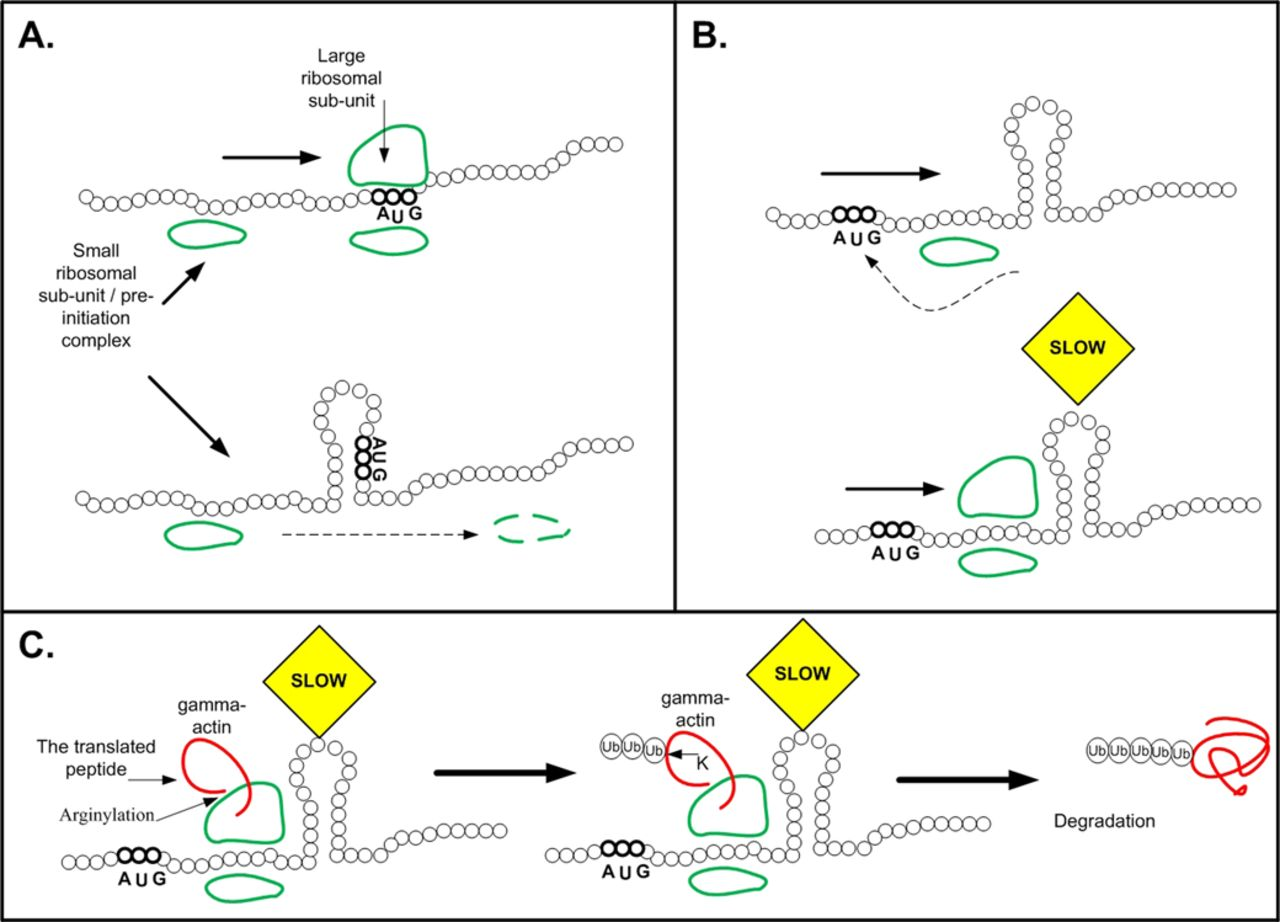
\includegraphics[width=1\textwidth]{chapters/Introduction/Figures/sec_str_rbs.jpg}
\caption[Secondary structure at the translation initiation site inhibits translation.]{\textbf{Secondary structure at the translation initiation site inhibits translation. (A) } The start codon AUG is recognised by the pre-initiation complex if the secondary structure is weak (top) but fails to do so in presence of a strong structure (bottom). \textbf{(B)} Presence of strong structure downstream of translation initiation site prevents the movement of pre-initiation complex (top) which could improve translation efficiency by improving ribosomal allocation (bottom). \textbf{(C)} Such downstream structures could influence post-translation modification by slowing down the ribosome. For example: lysin residues in arginylated gamma actin are exposed due to slow translation and undergo ubiquitination. Figure from Tuller and Zur, (2011) (Creative Commons license: CC BY ) }%the List of Figures because of the *}
\label{fig:sec_str_rbs}
\end{figure}



\paragraph{Computation of minimum free energy (MFE) and suboptimal structures}
Thermodynamically, an RNA structure with the lowest Gibbs free energy is the most stable. This energy is called minimum free energy. Thermodynamic ensembles usually follow the principle of locality, which says that interactions occur only between neighbouring particles. For example: In the Ising model of magnetism, spin interactions happen only between the nearest particles. Similarly, MFE is also calculated by using so called 'Turner parameters' \cite{turner2009nndb} in a nearest neighbouring model and a set of recursive equations called Zuker's algorithm \cite{zuker1981optimal}. However, the accuracy of the computed MFE is only within $5-10\%$ and a large number of alternate RNA structures lie within $5-10\%$ of the predicted global minimum \cite{eddy2004rna}. This prompts us to calculate some other free energies for different suboptimal conformations that RNA may achieve in a near thermodynamic equilibrium. Furthermore, depending on the criteria to pick an \textit{optimal} sturcture from a Boltzmann's ensemble, suboptimal structures may not lie near the thermodynamic equilibrium at all. For example: Ding \textit{et al.} \cite{ding2005rna}  found that structures tend to form clusters in a Boltzmann's ensemble. Instead of free energy, if we use these clusters as a criteria for sampling, then structure that has a minimum distance from all clusters is the optimial structure \cite{lorenz2016predicting}. This structure is also known as centroid structure and other structures around the centroid may as well be regarded as suboptimal.



There were some early attempts to compute suboptimal structures for example, by Zuker \cite{zuker1989finding} and Waterman \textit{et al.} \cite{waterman1985dynamic}. However, the backtracing procedure in their algorithms was not efficient enough to compute energies for longer RNA molecules. This problem was solved by McCaskill \cite{mccaskill1990equilibrium} by proposing an efficient algorithm to compute energy through a partition function which has the same time complexity as Zuker's algorithm for MFE $(\mathcal{O}(n^{3}))$.

\paragraph{Partition function and base pairing probabilities}
Consider a structure $s$ of an RNA molecule with free energy $E(s)$. In a thermodynamic ensemble of different structures at equilibrium, using the principle of maximum entropy, we see that the probability that the given RNA has the structure $s$ follows a Boltzmann distribution:

\begin{equation}
    p(s) \propto e^{-\beta E(s)}
\end{equation}

where $\beta$ is called 'thermodynamic beta' and equals $1/k_B T$, where $k_B$ is the Boltzmann's constant and $T$ is the absolute temperature (Subsection \ref{subsection:sim_anneal} Simulated annealing ). Since sum of probabilities over set of all structures $\Xi$, must be equal to unity, we have:

\begin{equation}
\begin{aligned}
    \sum_s p(s) &= \frac{1}{Z} \sum_{s\in\Xi} e^{-\beta E(s)}  = 1  \\
    Z &= \sum_{s\in\Xi} e^{-\beta E(s)} 
\end{aligned}
\label{eqn:part_func}
\end{equation}

The quantity $Z$, which plays a role of normalisation of probabilities, is called the \textit{canonical partition function}. Many thermodynamic parameters of interest can be derived from $Z$, for example, free energy $G$ of RNA in terms of $Z$ is given by:

\begin{equation}
\label{eqn:free_en}
    G = -\frac{1}{\beta} \ln(Z)
\end{equation}

The efficient dynamic programming to enumerate $Z$ was proposed by McCaskill \cite{mccaskill1990equilibrium} with time complexity of $\mathcal{O}(n^{3})$. This method is essentially a recursive decomposition of $Z$ similar to Zuker's algorithm only difference being the addition in Zuker's relation are now substituted by product because free energies are additive. If $E$ is the total free energy and $E_L$ are the energy contributions from various types of loops (hairpin, stacked pair, bulges, interior loops, multiloops) in a structure, then:

\begin{equation}
    E = \sum_L E_L
    \label{eqn:free_en_add}
\end{equation}

If we suppose the term $Q_{ij}^b$ accounts for all loops $L$ enclosed by $i,j$, we see that additivity of free energy (Equation \ref{eqn:free_en_add}) implies a multiplicative contribution to the partition function (\ref{eqn:part_func}) which gives the following recursive equation :

\begin{equation}
    Q_{ij}^b = \sum_L e^{-\beta E_L} \prod_{i<h<k<j} Q_{hk}^b
    \label{eqn:mcc_restr_part}
\end{equation}

Using this restricted partition function term for loop contributions, the total partition function between $i^{th}$ and $j^{th}$ nucleotides ($Q_{ij}$) can now be written as:

\begin{equation}
    Q_{ij} = Q_{i j-1} + \sum_{i \leq k <j} Q_{i k-1} Q_{kj}^b
    %where, by convention, Q_{i, i} = Q_{i, i-1} = 1.
    \label{eqn:mcc_full}
\end{equation}

The full partition function of RNA with $N$ nucleotides is given by $Z = Q_{1N}$. Equations \ref{eqn:mcc_restr_part} and \ref{eqn:mcc_full} are McCaskill's recursions for partition function. Once $Z$ is known, the probability of any structure $s$ with free energy $E(s)$ is given by:

\begin{equation}
\label{eqn:prob_part_func}
    p(s) = \frac{1}{Z} e^{-\beta E(s)}
\end{equation}

The computational approach outlined above is very generic and can be used for other specific cases. For example: if we want to know the probability that $[i^{th}, j^{th}]$ nucleotides are paired, then we can modify Equation \ref{eqn:part_func}, where partition function is found by simply summing Boltzmann's factor over all structures $\zeta$ where $[i^{th}, j^{th}]$ nucleotides are paired ($\zeta \subseteq \Xi$, where $\Xi$ is the ensemble of structures):

\begin{equation}
    Z_p = \sum_{s\in\zeta} e^{-\beta E(s)}
\end{equation}

The base pairing probabilities are, given by equation \ref{eqn:prob_part_func} with an appropriately computed $Z$. % which is Z on the above equation.


%% Avoidance
\subsubsection{mRNA:ncRNA avoidance}
Recently, Umu et al \cite{Umu2016-zq} found that in bacteria and the archaea, the strength of interactions between mRNAs and non-coding RNAs (ncRNAs) anti-correlate with protein levels. These signals are particularly obvious at the translation initiation site, suggesting that there is an avoidance of inappropriate interactions for highly expressed proteins. However, from a large pool of mRNA and ncRNA, a complete avoidance of interactions is unlikely and a trade off exists between interactions and protein expression. Further, it is suggested that compartmentalisation should minimise these cross talk interactions in eukaryotes. Compartmentalisation has been a topic of considerable research and is linked with noise filtering in gene expression and cellular feedback process \cite{rao2002control, stoeger2016passive, banani2017biomolecular, dong2017shaping}. We now outline in brief, the necessary background to understand the computation of RNA interactions and mRNA:ncRNA avoidance.


\paragraph{Unpairing of bases and accessibility}
McCaskill’s equations \ref{eqn:mcc_restr_part} and \ref{eqn:mcc_full} for the partition function can also be `inverted' to find the probability that $[i^{th}, j^{th}]$ nucleotides are unpaired in the given ensemble. The energy required to unpair the nucleotides is called accessibility or opening energy. If $\kappa \subseteq \Xi$ is the set of all structures $s$ where $[i^{th}, j^{th}]$ nucleotides are unpaired, then the accessibility is given by :

\begin{equation}
\begin{aligned}
    E_{accessibility} &= E_{s \in \kappa} - E_{s \in \Xi}\\
    E_{accessibility} &= -\frac{1}{\beta}\ln{\frac{Z_{unpaired}}{Z}}
\end{aligned}
\end{equation}

The term $\frac{Z_{unpaired}}{Z} = p_u$ is the probability that $[i^{th}, j^{th}]$  nucleotides  are unpaired \cite{Bernhart2011-cc}. Since the pair $i,j$ may or may not be enclosed by a base pair $k,l$ $\ni$ $\forall$ $k,l :$ $ k < i  < j < l$ (Figure \ref{fig:part_fun_decomp}), this probability can be computed by McCaskill approach \cite{Bernhart2011-cc}. Accessibility prediction forms the basis of RNA:RNA interactions. 



\begin{figure}[htbp!]
\center
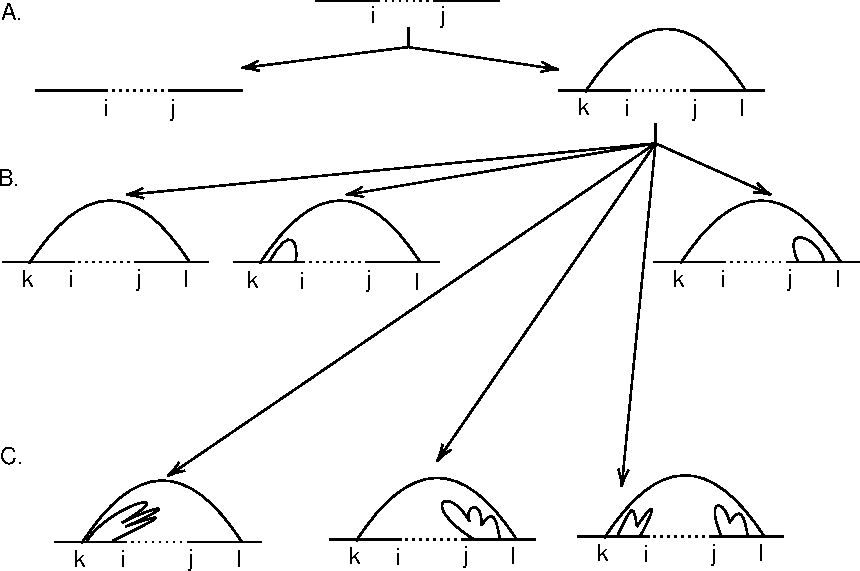
\includegraphics[width=1\textwidth]{chapters/Introduction/Figures/accs.pdf}
\caption[Decomposition of partition function to calculate unpairing probability of the region $(i,j)$ in a nucleotide sequence.]{\textbf{Decomposition of partition function to calculate unpairing probability of the region $[i,j]$ in a nucleotide sequence. (A)}  The interval [i,j] may either be enclosed by pair [k,l] (right) or may be open (left). \textbf{(B)} The enclosed pair may or may not contain an hairpin or \textbf{(C)} multiloops. The partition function $Z_{unpaired}$ is a sum of all these contributions.  Figure adapted from Bernhart \textit{et al.}, (2011)}%the List of Figures because of the *}
\label{fig:part_fun_decomp}
\end{figure}


% The exact equation to compute this probability and the accessibility in $\mathcal{O}(n^{3})$ time is given by Bernhart \textit{et al.}  with an algorithmic implementation in RNAplfold of ViennaRNA suite \cite{Lorenz2011-rg}. Accessibility prediction forms the basis of RNA:RNA interactions. 


\paragraph{RNA:RNA interactions} \label{subsec:rna_interac}
For two RNA molecules to interact and pair, most computational tools assume that this is  a two step process\textemdash unfolding of the RNA molecules at the target sites, followed by an actual interaction (hybridisation) \cite{Muckstein2006-ys}.
Thus, the total binding energy $\Delta G$ is the sum of the accessibility of the target site of the longer RNA molecule $\Delta G_{unpaired}$ and the subsequent interaction between the unfolded region of the interacting molecules $\Delta G_{int}$. $\Delta G_{unpaired}$ is computed by equation $1.8$, where as $\Delta G_{int}$ is computed through equation \ref{eqn:free_en} by replacing $Z$ with $Z_{int}$. For an interaction between nucleotides $[i, j]$ and $[i^*, j*]$ the partition function $Z_{int}$ is given by \cite{Muckstein2006-ys} (Figure \ref{fig:part_fun_interac}):





\begin{equation}
\begin{aligned}
    Z_{int} &= p_u[i,j] \sum_{i^*>j*} Z^I[i,j,i^*,j^*] \\
    where, \\
    Z^I[i,j,i^*,j^*] &= \sum_{\substack{i<k<j\\
    j*<k^*<i^*}} Z^1[i,k,i^*,k^*] e^{E_I(i,k,i^*,k^*)}
\end{aligned}
\end{equation}

with $E_I(i,k,i^*,k^*)$ as the free energy of the interior loop enclosed by $(i,k)$ and $(i^*,k^*)$ and $Z^1[i,k,i^*,k^*]$ contains at least one substructure between $(i,k)$ and $(i^*,k^*)$. 

\begin{wrapfigure}{r}{0.5\textwidth}
  \begin{center}
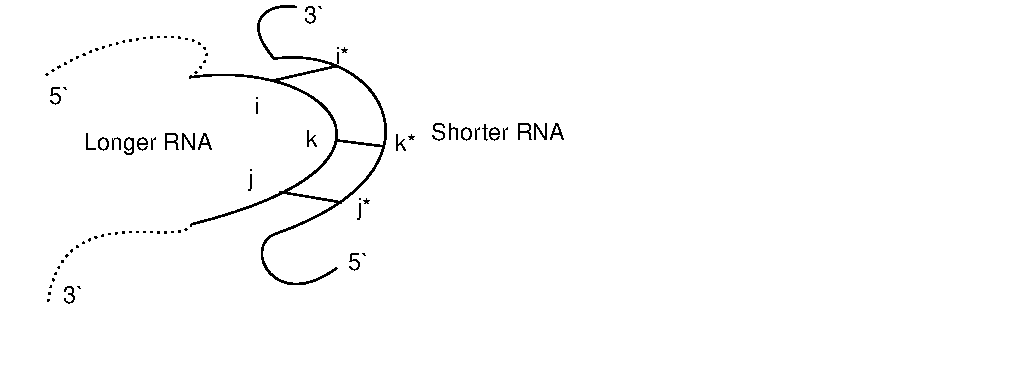
\includegraphics[width=0.7\textwidth]{chapters/Introduction/Figures/interac.pdf}
\caption[RNA:RNA interaction and notations used for partition function.]{\textbf{RNA:RNA interaction and notations used for partition function.} Full shape of longer RNA is not shown. The nucleotides between $[i,j]$ and $[i^*,j^*]$ may contain mismatches. Figure adapted from Muckstein \textit{et al.}, (2006). }%the List of Figures because of the *}
\label{fig:part_fun_interac}
  \end{center}
\end{wrapfigure}

The RNA:RNA interaction prediction mechanisms are still being actively refined because many RNA:RNA interactions have important regulatory functions. For example, in eukaryotes, microRNAs can reduce the levels of mRNAs by interacting with the $3^{\prime}$UTRs of the mRNA targets \cite{catalanotto2016microrna, valencia2006control}.










Apart from these general mRNA features which play a role in protein expression, several specific features also exist. For example: Cis-regulatory elements such as promoters and enhancers, interactions of mRNA with sRNA and miRNA as well as introns in $5^{\prime}$ UTR in eukaryotes. However, our discussion will be based around the general features only. 


A number of gene optimisation tools build a suitable cost or fitness function using a combination of these features. Typically, a genetic algorithm is then used to optimise the fitness. The synonymous mRNA sequence with the maximum fitness is regarded as the optimised mRNA sequence with optimal expression \cite{Villalobos2006-nx, Salis2009-dh, Raab2010-eg, Chung2012-zh, Terai2016-vp}. Despite being optimised on expression, the sequences may form aggregates, which cannot be used for further studies \cite{gustafsson2004codon, rosano2009rare}. This leads us to the discussion of optimising solubility. 
